
%(BEGIN_QUESTION)
% Copyright 2006, Tony R. Kuphaldt, released under the Creative Commons Attribution License (v 1.0)
% This means you may do almost anything with this work of mine, so long as you give me proper credit

A device called a {\it manometer} is a very simple and yet very precise pressure measuring instrument.  It works on the principle of a differential pressure displacing a vertical liquid column.  The distance between the tops of the two liquid columns is proportional to the difference in pressure applied to tops of the two vertical tubes.  This is where we get pressure units of ``inches/centimeters of water column'' and ``inches/centimeters/millimeters of mercury'' -- from the operation of a manometer:

$$\includegraphics[width=15.5cm]{i00160x01.eps}$$

Explain how this instrument may serve as a standard for pressure measurement, just as a deadweight tester may serve as a standard for pressure generation.  To phrase this question in the negative, what would have to change in order to affect the pressure measurement accuracy of a manometer?

\underbar{file i00160}
%(END_QUESTION)





%(BEGIN_ANSWER)

The accuracy of a manometer is fixed by two fundamental variables, both of which are quite constant:

\medskip
{\item{} The density (mass per unit volume) of the manometer liquid
{\item{} The gravity of Earth
\medskip

So long as these two variables do not change, neither will the accuracy of the manometer.

%(END_ANSWER)





%(BEGIN_NOTES)

So long as these two variables do not change, neither will the accuracy of the manometer.  The most likely of the two variables to change is the liquid density, and this by temperature change and/or contamination.  So long as the manometer is kept at a fairly constant room temperature, and the liquid is kept free of impurities, the manometer should be very accurate.  Like deadweight testers and any other instruments dependent on Earth's gravity, manometers need to be maintained as close as possible to a perfectly vertical position in order to be accurate.

%INDEX% Measurement, pressure: manometer

%(END_NOTES)


